% This is a sample LaTeX input file.  (Version of 11 April 1994.)
%
% A '%' character causes TeX to ignore all remaining text on the line,
% and is used for comments like this one.

\documentclass[11pt]{article}      % Specifies the document class
\usepackage{amsfonts,amssymb,amsmath}
\topmargin-0.2in
\textheight9.0in
\oddsidemargin-0.2in
\evensidemargin-0.2in
\textwidth6.5in

\usepackage{graphicx} % Required for inserting images
\usepackage{booktabs}
\usepackage{subcaption}
\usepackage{xcolor}  

\usepackage{listings}
\lstset{
	basicstyle=\footnotesize\ttfamily,
	columns=flexible,
	breaklines=true,
	commentstyle=\color{red},
	keywordstyle=\color{black}\bfseries}

\newcommand{\mZ}{\mathbb Z}
\newcommand{\mR}{\mathbb R}
\newcommand{\mC}{\mathbb C}
\newcommand{\mQ}{\mathbb Q}
\newcommand{\ep}{\epsilon}
\begin{document}             % End of preamble and beginning of text.

%\thispagestyle{empty}
\begin{center}
{\bf\large HW1(FEA): Appiah Francis}\\
\vspace{0.05in}
\end{center}
\noindent {\sf Instructions:}
{\em 
\begin{itemize}
\item [1.)] There are in total 85 points. Submit your report as a single PDF document to gradescope (linked via LMS); And mark the location(s) of your work for each problem,  as instructed during submission.
\item [2.)] If AI tools are used to assist you with this homework, state what \& how AI tools are used.
\item [3.)] Part II of this homework set is for numerical implementation. Your report for this part should consist of
{\sf 
\begin{itemize}
\item  Brief description of the problem
\item Results such as data, graphs etc. Try to avoid attaching large set of data unless it is really necessary.
\item Discussion, comments, explanation and conclusion on your numerical observations. This part is equally important as your computer codes and the data you collect, and it helps with understanding concepts, algorithms, or other relevant issues not discussed during lectures. 

\item Computer codes printouts, attached to the very end of your entire report. Program text is expected to be well structured so others (at least from the same class) can read it without much difficulty. Add extra comments if needed.
\end{itemize}
}


\end{itemize}
}

\begin{enumerate}

\item[]{\bf Part -1: Polynomial space $P^1(I)$.} (This problem is {\bf not collected} for grading.)

Let $I=[x_0, x_1]$. Verify by direct calculation that  the nodal basis functions 
\begin{equation}
\lambda_0(x)=\frac{x_1-x}{x_1-x_0}, \quad \lambda_1(x)=\frac{x-x_0}{x_1-x_0}
\end{equation}
for $P^1(I)$ (the set of linear polynomials on $I$) satisfy
\begin{equation}
\lambda_0(x)+\lambda_1(x)=1,\quad x_0\lambda_0(x)+ x_1\lambda_1(x)=x.
\end{equation}
Is this a surprise to you, especially if you know that $\lambda_i(x_j)=\delta_{ij}, i, j =0, 1?$ 

 
 
\item[]{\bf Part 0: Acknowledgement if relevant:} e.g., significant help/assistance from other people, use of reference materials and/or AI tools etc.
 
\newpage
\item[]{\bf Part I: Variational/weak formulation.}  Consider the following two-point boundary value problem:
\begin{displaymath}
{\textrm{(D)}} \;\;\left\{
\begin{array}{ll}
-(p(x)u'(x))'+q(x)u(x)=f(x),& x\in(0,1)\\
u(0)=u(1)=0&
\end{array}
\right.
\end{displaymath}
where $f(x), p(x), q(x)$ are given smooth functions (such as $f, q\in C([0, 1])$, and $p\in C^1([0, 1])$) and $p(x)>0$, $q(x)\geq 0$.
Suppose we know (D) has a unique solution $u\in C^2([0, 1])$.

\begin{enumerate}
%-- Weak formula
\item ({\bf 8 points})
Derive a variational/weak formulation (V) for (D):
\begin{displaymath}
{\textrm{(V)}} \;\;\left\{
\begin{array}{l}
\mbox{look for} \; u\in W, \; \mbox{such that}\\
a(u, v)=(f, v),\qquad \forall v\in W.
\end{array}
\right.
\end{displaymath}

You would need to {\bf specify} the trial and test space $W$ ({\em which may or may not be the same as the one used in class}) and 
$a(u, v)$. One requirement is that 
$a(u, v)$ is symmetric, namely $a(u, v)=a(v, u)$. {\bf Justify} your choice of each component (i.e. trial space, test space, $a(u,v)$) in the variational formulation ({\em refer to lecture notes}). \\


{\em Note: 
$C^n([0,1])=\{v: v, v', \cdots, v^{(n)} \;\textrm{are continuous functions on} \; [0,1]\}.$
When $n=0$, we also use $C([0,1])=C^0([0,1])$. $a(u,v)$ is some mapping from $W\times W$ to $\mathbb R$.
} 

{\bf Solution:}
To derive the variational/weak formulation (V) for (D) we multiply equation (D) by a test function $v(x)$ and integrate with respect to $x$.
\begin{align}\label{eqn:testfunc}
	-\int_{0}^{1}(p(x)u'(x))'v(x)\,dx + \int_{0}^{1}(q(x)u(x))v(x)\,dx = \int_{0}^{1}f(x)v(x)\,dx.
\end{align}
Applying integration by parts on the first term of equation~(\ref{eqn:testfunc}), we have 
\begin{align}
	\int_{0}^{1}(p(x)u'(x))v'(x)\,dx &-(p(1)u'(1))v(1) + (p(0)u'(0))v(0) \\
	&+ \int_{0}^{1}(q(x)u(x))v(x)\,dx = \int_{0}^{1}f(x)v(x)\,dx. \nonumber
\end{align}
We impose $v(0) = 0, v(1)=0$, this results in
\begin{align}\label{eqn:bilinear}
	(pu',v') + (qu,v) = (f,v).
\end{align}
Define $a(u,v) = (pu',v') + (qu,v)$, then 
$$a(u,v) = (f,v).$$
Since $u\in C^2([0,1])$, then $u\in L^2([0,1])$. This implies that for equation~(\ref{eqn:bilinear}) to be well-defined then we choose the  test space $W$ as
\begin{align}
	v\in W = \{v: v\in C([0,1]), v,v' \in L^2([0,1]), v(0)=v(1)=0\},
\end{align}
ensuring that boundary conditions are strongly imposed through the space. Hence $u$ also belongs to the space $W$. The trial space will be the same as the test space. The variational/weak form (V) is 
\begin{displaymath}
	{\textrm{(V)}} \;\;\left\{
	\begin{array}{l}
		\mbox{look for} \; u\in W, \; \mbox{such that}\\
		a(u, v)=(f, v),\qquad \forall v\in W.
	\end{array}
	\right.
\end{displaymath}
where
$$a(u,v) = (pu',v') + (qu,v).$$
We need to also justify that $a(u,v)$ is symmetric, thus $a(u,v) = a(v,u)$
\begin{align*}
	a(u,v) &= (pu',v') + (qu,v),\\
	&= \int_{0}^{1}(p(x)u'(x))v'(x)\,dx + \int_{0}^{1}(q(x)u(x))v(x)\,dx,\\
	& = \int_{0}^{1}(p(x)v'(x))u'(x)\,dx + \int_{0}^{1}(q(x)v(x))u(x)\,dx,\\
	&= (pv',u') + (qv,u) = a(v,u).
\end{align*}
%-- FEM
%
\item ({\bf 20 points}) Now we want to formulate a finite element method (FEM) for (V).  Given a partition of $[0,1]$: $0=x_0<x_1<\cdots<x_{j-1}<x_j<\cdots<x_N<x_{N+1}=1$, and let $I_j=[x_{j-1}, x_j]$, $h_j=x_j-x_{j-1}$ and $h=\max_j h_j$. We further define a finite element space 
$$
W_h=\{v(x)\in W: v(x)|_{I_j}\in P^1(I_j), \forall j\}.
$$
A FEM for solving (V) can then be formulated as follows:

\begin{displaymath}
{\textrm{(FEM)}} \;\;\left\{
\begin{array}{l}
\mbox{look for} \; U_h(x)\in W_h, \; \mbox{such that}\\
a(U_h, v)=(f, v),\qquad \forall v\in W_h.
\end{array}
\right.
\end{displaymath}

If $U_h(x)=\sum_{j=1}^{N} c_j\phi_j(x)$, where $\{\phi_j\}_{j=1}^N$ are the nodal basis functions as discussed in class,  the FEM formulation can be converted into an  algebraic system:
\begin{equation}
\label{eq:1}
{\bf A c}={\bf F},
\end{equation}
%

with ${\bf A}=(a_{ij})\in{\mathbb R}^{N\times N}$, ${\bf c}=[c_1, \cdots, c_{N}]^T\in{\mathbb R}^N$ and ${\bf F}=[(f, \phi_1), \cdots, (f, \phi_N)]^T\in{\mathbb R}^N$.

\begin{itemize}
%
\item[]b.1) Show that $U_h(x)\in W_h$ solves (FEM), if and only if $U_h(x)\in W_h$ solves the following:
\begin{displaymath}
{\textrm{(ALT)}} \;\;\left\{
\begin{array}{l}
\mbox{look for} \; U_h(x)\in W_h, \; \mbox{such that}\\
a(U_h, \phi_j)=(f, \phi_j),\qquad j=1, 2, \cdots, N.
\end{array}
\right.
\end{displaymath}
{\bf Solution:}
Assume $U_h(x) \in W_h$ solves (FEM). Since $\{\phi_j\}_{j=1}^N$ are the nodal basis functions then $\phi_j \in W_h$ for all $j$. We pick $v=\phi_j$ for $j=1,2,\ldots,N$. Hence $U_h(x)$ solves (ALT). We show that the reverse also hold, that is if $U_h(x)$ solves (ALT) then it solves (FEM). Since $\{\phi_j\}_{j=1}^N$ is a basis for $W_h$, any function in the space $W_h$ can be written as 
\begin{align*}
	v(x) =\sum_{j=1}^{N} v_j\phi_j(x) .
\end{align*} 
This implies that
\begin{align*}
	a(U_h,v) &= a(U_h,\sum_{j=1}^{N} v_j\phi_j)\\
	 &= \sum_{j=1}^{N} v_j(a(U_h,\phi_j))\\
	&\overset{solves (ALT)}{=} \sum_{j=1}^{N} v_j(f,\phi_j)\\ 
	&= a(f,\sum_{j=1}^{N} v_j\phi_j) = (f,v).
\end{align*}

%
\item[]b.2) Write down the formula for $a_{ij}$ in terms of $p(x), q(x)$ and $\{\phi_j(x)\}_{j=1}^N$.\\

{\bf Solution:} From the (FEM) equation we have
$$a(U_h,\phi_j) = (f,\phi_j), \quad j = 1,2,\ldots,N.$$ We have $U_h(x) = \sum_{j=1}^{N}c_j\phi_j(x)$, this implies that
\begin{align*}
	a(U_h,\phi_j) &= (pU'_h,\phi'_j) + (qU_h,\phi_j) , \quad j = 1,2,\ldots,N.\\
	&=(p(\sum_{j=1}^{N}c_j\phi_j)',\phi'_i) + (q(\sum_{j=1}^{N}c_j\phi_j),\phi_i)\\
	&=\sum_{j=1}^{N}(p\phi_j',\phi'_i)c_j + \sum_{j=1}^{N}(q(\phi_j),\phi_i)c_j\\
	&=\sum_{j=1}^{N}[(p\phi_j',\phi'_i) + (q(\phi_j),\phi_i)]c_j
\end{align*}
Hence 
$$a_{ij} = (p\phi_j',\phi'_i) + (q(\phi_j),\phi_i).$$
%
\item[]b.3) Show that ${\bf A}$ is symmetric positive definite. \\
{\bf Solution:}
$A$ is positive definite if $$\mathbf{c}^T{\bf A}\mathbf{c} >0 \quad \forall\, \mathbf{c}\in\mathbb{R}^N.$$
For all $\mathbf{c} \in\mathbb{R}^N$ and $\mathbf{c} \neq\mathbf{0}$,
\begin{align*}
	\mathbf{c}^T {\bf A} {\bf c} &= \sum_{j=1}^{N}\sum_{i=1}^{N}c_jc_ia_{ij}\\
	&=\sum_{j=1}^{N}\sum_{i=1}^{N}c_jc_i\bigg[(p\phi'_j,\phi'_i) + (q\phi_j,\phi_i)\bigg]\\
	&=\sum_{j=1}^{N}\sum_{i=1}^{N}c_jc_i\big[(p\phi'_j,\phi'_i)\big]  + \sum_{j=1}^{N}\sum_{i=1}^{N}c_jc_i \big[(q\phi_j,\phi_i)\big]\\
	&=\left(p\left(\sum_{i=1}^{N}c_j\phi_j\right)',\left(\sum_{i=1}^{N}c_i\phi_i\right)'\right) + \left(q\left(\sum_{i=1}^{N}c_j\phi_j\right),\left(\sum_{i=1}^{N}c_i\phi_i\right)\right)
\end{align*}
Let $v = \sum_{j=1}^{N}c_j\phi_j$, then 
\begin{align*}
\mathbf{c}^T {\bf A} {\bf c} &=(pv',v') + (qv,v), \\
&= \int_{o}^{1}p(x)(v'(x))^2\, dx + \int_{o}^{1}q(x)(v(x))^2\, dx \geq 0, \,\text{ since } p(x)> 0, q(x) \geq 0.
\end{align*}
%We need to check that for ${\bf c}^T {\bf Ac} = 0$, implies ${\bf c} = {\bf 0}$, which will be a contradiction
Now if ${\bf c}^T {\bf Ac} = 0$, this implies that $v'(x) = 0$ and since $v(x)$ is continous on $[0,1]$, $v(x)$ = constant on $[0,1]$. From boundary condition $v(0) = v(1) = 0$, implies $v(x)\equiv 0$ for $x\in[0,1]$. Hence $\sum_{j=1}^{N}c_j\phi_j =0$ , this implies $c_j = 0$ for $i = 1,2,\ldots,N$ since $\{\phi_j\}_{j=1}^N$ are basis. This implies that 
$$\mathbf{c}^T {\bf A} {\bf c} = 0 \iff {\bf c} = {\bf 0}.$$
This shows that 
$\mathbf{c}^T {\bf A} {\bf c} > 0,$ hence ${\bf A}$ is positive definite.
To show that ${\bf A}$ is symmetric we need to show that $a_{ij} = a_{ji}$. 
\begin{align}
	a_{ij} &= (p\phi'_j,\phi'_i) + (q\phi_j,\phi_i)\\
		&= \int_{0}^{1}(p(x)\phi_j'(x))\phi_i'(x)\,dx + \int_{0}^{1}(q(x)\phi_j(x))\phi_i(x)\,dx,\\
	& = \int_{0}^{1}(p(x)\phi_i'(x))\phi_j'(x)\,dx + \int_{0}^{1}(q(x)\phi_i(x))\phi_j(x)\,dx,\\
	&= (p\phi'_i,\phi'_j) + (q\phi_i,\phi_j) = a{ji}.
\end{align}
Hence ${\bf A}$ is symmetric positive definite.

\item[]b.4) If both $U_h^1, U_h^2 \in W_h$ are finite element solutions to (FEM), show that $U_h^1=U_h^2$. {\em This implies that  the finite element solution $U_h\in W_h$  does not depend on the choice of the basis for $W_h$.}\\
{\bf Solution:} If $U^1_h$ and $U^2_h$ are finite element solutions to (FEM) then 
\begin{align*}
	a(U_h^1 ,v) = (f,v),\\
	a(U_h^2,v) = (f,v).
\end{align*}
This implies that
\begin{align}
	a(U^1_h - U_h^2,v) = 0, \quad \forall\; v\in W_h.
\end{align}
We take $v = U^1_h - U^2_h$, then 
\begin{align*}
	a(U^1_h - U_h^2,U^1_h - U^2_h) = 0.
\end{align*}
let us define $w = U^1_h - U^2_h$, then  
\begin{align*}
	a(w,w) = (pw',w') + (qw,w) = 0
\end{align*}
\begin{align}
	(pw',w') + (qw,w) = 0\\
	\int_{0}^{1}p(w'(x))^2 \;dx + \int_{0}^{1}q(w(x))^2 \;dx = 0
\end{align}
since $p(x)>0$ and $q(x)\geq0$ then 
\begin{align}
	p(x)(w'(x))^2 + q(x)(w(x))^2 = 0, \; x\in [0,1].
\end{align}
For the case where $q(x) = 0$, then 
$w'(x) = 0 ,\; x\in [0,1]$. It follows that $w(x)$ is constant on $[0,1]$ which together with the boundary condition $U_h^1(0)=U_h^2(0) = 0$ gives $U_h^1(x) = U_h^1(x)$, for all $x\in[0,1]$. In the case $q(x)>0$ then $w(x) = 0$ and $w'(x) = 0 ,\; x\in [0,1]$. From the same argument we ahow that $U_h^1(x) = U_h^1(x)$.  This implies that If both $U_h^1, U_h^2 \in W_h$ are finite element solutions to (FEM), then $U_h^1=U_h^2$.
\end{itemize}
{\em Reminder:  keep in mind that the coefficient function $q(x)$ may be zero.}
\end{enumerate}

%--- coding
\item[]{\bf Part II: Implementation.}  Write a computer code to compute the FEM approximation $U_h(x)$ for $u(x)$ as defined in {\bf Part I}. In the computation, we use
\begin{itemize}
%
\item {\sf Parameters and the exact solution:} $p(x)=3$, $q(x)=2$, and the exact solution is
\begin{equation}
u(x)=x(x-1)(\sin(5x)+3e^x).
\label{eq:exa}
\end{equation}
You would need to derive the formula for the load function $f(x)$.
%
\item {\sf Mesh:} 
nonuniform but structured meshes
\begin{displaymath}
h_{j}=
\left\{
\begin{array}{ll}
0.9\Delta x, & {\textrm {for odd}}\; j\\
1.1\Delta x,& {\textrm {for even}}\; j,
\end{array}
\right.
\end{displaymath}
with $\Delta x=\frac{1}{N+1}$. We compute for $N+1=10, 20, 40, 80, 160, 320$.
%
\item {\sf Precision:} double precision computation ({\sf this is by default in matlab})
%
\item {\sf How to compute the errors and convergence orders:}


(1.) Let $e_h(x)=U_h(x)-u(x)$, then the error in  the {\bf $L^2$ norm} $||e_h(\cdot)||_{L^2(0,1)}$ can be computed as
{\small
\begin{align*}
||e_h(\cdot)||_{L^2([0,1])}:=&\left(\int_0^1 (e_h(x))^2dx\right)^{1/2}= \left(\sum_{j=1}^{N+1}||e_h(\cdot)||^2_{L^2(I_j)}\right)^{1/2}\\
\approx&\left(\sum_{j=1}^{N+1}\sum_{m=1}^{M}\left(e_h(x_{j-1}+\frac{h_j}{M} m)\right)^2 \frac{h_j}{M}\right)^{1/2},
\end{align*}
}
the error in the {\bf  $L^{\infty}$ norm} can be computed as
{\small
\begin{align*}
||e_h(\cdot)||_{L^\infty([0,1])}:=&\max_{x\in[0,1]}|e_h(x)|=\max_{1\leq j\leq N+1} ||e_h(\cdot)||_{L^\infty(I_j)}\\
\approx &\max_{1\leq j\leq N+1}\left[\max_{1\leq m\leq M}|e_h(x_{j-1}+\frac{h_j}{M} m)|\right],
\end{align*}
}
and the error in the {\bf energy norm} is defined as:
$$
||e_h(\cdot)||_{h}=||e_h'(\cdot)||_{L^2([0,1])}.
$$

you can use $M=3$ in your computation.
%

(2.) the convergence order in the $L^2$ norm can be computed as
$$\frac{\log\left(||e_{h}(\cdot)||_{L^2([0,1])}/||e_{\frac{h}{2}}(\cdot)||_{L^2([0,1])}\right)}{\log (2)}.$$
Similarly, you can compute the convergence order in $L^\infty$ norm and in the energy norm.

\smallskip
{\em Notation: if $U_h(x)$ is the numerical solution with $\Delta x=\frac{1}{N+1}$, then $U_{\frac{h}{2}}(x)$ is the numerical solution with $\Delta x=\frac{1}{2(N+1)}$.}\\
{\bf Solution:} We already showed from Part I that if $\{\phi_j\}_{j=1}^N$ is a set of basis then $U_h(x) \in W_h$ solves (FEM) if and only if $U_h(x)$ solves 
\begin{displaymath}
	\left\{
	\begin{array}{l}
		\mbox{look for} \; U_h(x)\in W_h, \; \mbox{such that}\\
		a(U_h, \phi_j)=(f, \phi_j),\qquad j=1, 2, \cdots, N.
	\end{array}
	\right.
\end{displaymath}
We implement (FEM) by defining a continous piecewise linear finite element space 
$$
W_h=\{v(x)\in W: v(x)|_{I_j}\in P^1(I_j), \forall j\}.
$$
where $P^1(I_j)$ is a set of polynomials of degree up to 1.
Let $U_h(x) = \sum_{j=1}^{N}c_j\phi_j$ , then we convert (FEM) into an algebraic system 
$${\bf Ac} = {\bf F},$$ where the components of ${\bf A} = a_{ij}$ is define as  
$$a_{ij} = (p\phi_j',\phi'_i) + (q\phi_j,\phi_i),$$
and $$F_i = (f,\phi_i), \quad i = 1,2,\ldots,N.$$
$p(x) = 3, \, q(x) = 2$, then 
$$a_{ij} = 3(\phi_j',\phi'_i) + 2(\phi_j,\phi_i).$$ The Matrix $A$ is tri-diagonal, thus $a_{ij} \neq$ when $j = i-1,i,i+1$. Let us define 
\begin{align*}
	\tilde{a}_{ij} &\overset{\text{def}}{=}(\phi'_j,\phi'_i),\\
	m_{ij} &\overset{\text{def}}{=}(\phi_j,\phi_i),
\end{align*}
where
\begin{align*}
	\tilde{a}_{i,i}  &= \frac{1}{h_i} + \frac{1}{h_{i+1}},\,\tilde{a}_{i,i-1} = -\frac{1}{h_i},\,\tilde{a}_{i,i+1} = -\frac{1}{h_{i+1}} \\ 
	m_{i,i}  &= 1/3(h_i + h_{i+1}),\,m_{i,i-1} = 1/6h_i ,\,m_{i,i+1} =1/6 h_{i+1} . 
\end{align*}
Hence 
\begin{align*}
	a_{i,i} &= 3(\frac{1}{h_i} + \frac{1}{h_{i+1}}) + 2/3(h_i + h_{i+1}),\\
	a_{i,i-1} &= -\frac{3}{h_i} +\frac{ h_i}{3},\\
		a_{i,i+1} &= -\frac{3}{h_{i+1}} +\frac{ h_{i+1}}{3}.
\end{align*} 
To calculate the load vector 
\begin{align*}
	F_i = (f,\phi_i) = f_im_{ij} ,\quad i,j =1,2,\ldots,N.
\end{align*}
This implies that 
$$
F_i = f_{i+1}\frac{h_{i+1}}{6} + f_i\frac{h_i + h_{i+1}}{3} + f_{i-1}\frac{h_{i}}{6}, \quad i =1,2,\ldots,N,
$$
where $f_i = f(x_i)$. From the equation (D) 
$$f(x) = -3u''(x) + 2u. $$ Given an exact solution $$u(x)=x(x-1)(\sin(5x)+3e^x),$$
we have
\begin{align*}
	u'(x) &= x(x-1)(5\cos(5x)+3e^x) + (2x-1)(\sin(5x)+3e^x),\\
	u''(x) &= x(x-1)(-25\sin(5x)+3e^x) + 2(2x-1)(5\cos(5x)+3e^x)+ 2(\sin(5x)+3e^x).
\end{align*}
The error function 
$$e_h(x) = U_h(x) - u(x),$$
where 
$$
U_h(x) = c_{j-1}\phi_{j-1} + c_j\phi_j, \, \text{ for } x\in I_j, \, j = 1,2,\ldots,N,
$$
\begin{align*}
	\phi_{j-1} &= \frac{x_j - x}{h_j}, \qquad  x\in I_j,\\
	\phi_j &= \frac{x-x_{j-1}}{hj},  \qquad  x\in I_j.
\end{align*}
Hence 
$$
U_h(x) = c_{j-1}( \frac{x_j - x}{h_j}) + c_j(\frac{x-x_{j-1}}{hj}), \, \text{ for } x\in I_j, 
$$
with $c_0 = c_{N+1} = 0.$ The first derivative of $U_h(x)$ is given as
$$
U'_h(x) = \frac{(c_j - c_{j-1})}{h_j}.
$$
We form matrix $A$ and vector ${\bf F}$, then we solve for ${\bf c}$. We then use ${\bf c}$ to form $U_h(x)$ on each mesh element $I_j$. We can then calculate the error in $L^2 , L^{\infty}$  norm and the energy norm.
\end{itemize}


Based on what you get from your computer code:
\begin{enumerate}
\item ({\bf 4 points})
 Within one graph, plot the error function $e_h(x)$ for $N+1=10, 20, 40$. In a separate graph, present the semi-log plots of $g(x)=|e_h(x)|$ for $N+1=10, 20, 40$. 
    
    {\em Note: The semi-log is in $g(x)$, not in $x$. Moreover, $g(x)$ is defined everywhere in $(0,1)$, you should sample several points in each mesh element $I_j$  when plotting the error function. This is different from visualization of solutions from finite difference methods.}. \\
{\bf Solution: }
\begin{figure}[htbp]
	\centering
	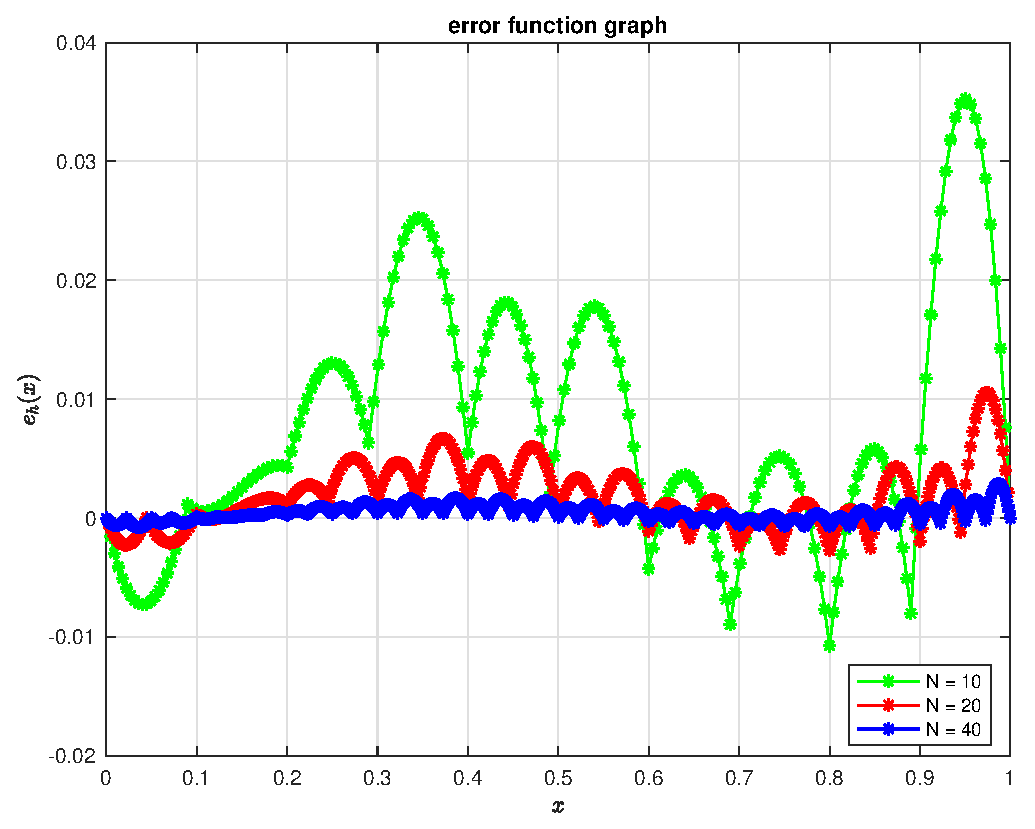
\includegraphics[width=0.55\textwidth]{img/errorgraph.eps}
	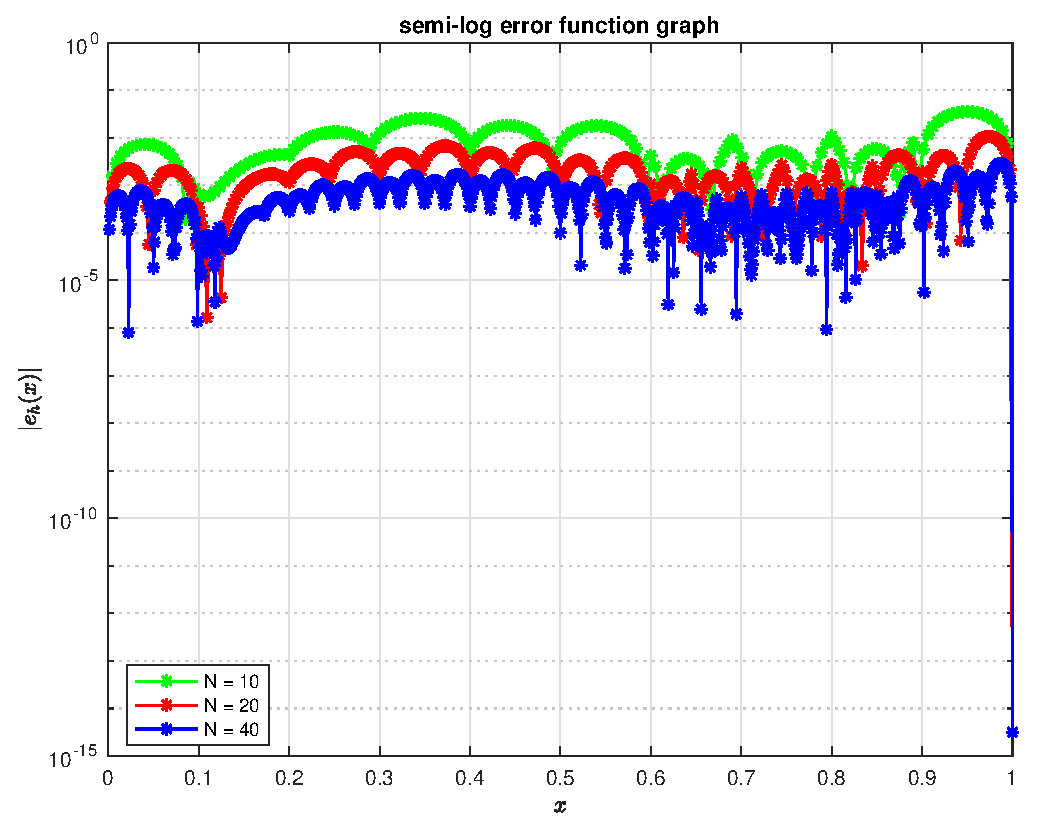
\includegraphics[width=0.55\textwidth]{img/semilogerrgraph.eps}
	\label{fig:N3}
\end{figure}
\item ({\bf 15 points})
Report the errors in $L^2$ norm, $L^\infty$ norm, and the energy norm, as well as the respective convergence orders for $N+1=10, 20, 40, 80, 160, 320$. Please organize your data into a table as illustrated in Table \ref{tab1}, and your data should be presented in the same format as in Table \ref{tab1}. ({\em Latex source file is shared in LMS.}) 

{\em\small Notes:
\begin{itemize}
\item For completeness, report 
which linear solver is used to solve the linear system (\ref{eq:1}).
\item For large N, you may want to consider working with the sparse form of a matrix for better efficiency in storage and computation.
 \item The actual data in Table \ref{tab1} is only for illustration and it is not related to our problem here.
 \item Using the number 2.11E-02 as an example, do not report it as 0.02. Too many significant digits are lost.
 \end{itemize}
 }
 
\begin{table}[!h]
\caption{Errors and convergence orders when $p=3, q=2$ and $u=x(x-1)(\sin(5x)+3e^x)$}
\vspace{0.1in}
\centering
\begin{tabular}{|c|c|c| c| c| c| c|}
\hline
 $N+1$&  $||e_h(\cdot)||_{L^2([0,1])}$ & Order  & $||e_h(\cdot)||_{L^\infty([0,1])}$ & Order& $||e_h(\cdot)||_h$& Order \\
 \hline
     10 & 1.30E-02 & - & 3.30E-02 & - & 4.60E-01 &- \\
     20 & 3.26E-03 & 2.00&9.66E-03   & 1.77   & 2.24E-01 &1.04\\
     40 & 8.09E-04  & 2.01 & 2.61E-03   & 1.89 & 1.11E-01 &1.02\\
     80 & 2.01E-04  & 2.01 & 6.78E-04   & 1.94 & 5.49E-02 &1.01\\
     160 & 5.02E-05   & 2.00 & 1.73E-04   &1.97  & 2.73E-02 &1.01\\
     320 &1.25E-05   & 2.00  & 4.36E-05   & 1.99 & 1.36E-02 &1.00\\
\hline
\end{tabular}
\label{tab1}
\end{table}

\item ({\bf 10 points}) 
Now we consider an example with variable coefficients, namely $p(x)=1+x$, and $q(x)=0$. The exact solution is given by  equation \eqref{eq:exa}. Note that you would need to derive the source function $f$ and re-compute the matrix $A$.\\
{\bf Solution: } For $p(x) = 1+x$ and $q(x) = 0$, we have 
\begin{align*}
	f(x) &= -(p(x)u'(x))', \\
	&=-(1+x)u'' - u'.
\end{align*}
\begin{itemize}
\item[(c.1)] Hand calculate, explicitly, the entry  $a_{ij}$ of $A$;\\
{\bf Solution:}
Computing the matrix A, and since $q(x)=0$ we have that
\begin{align}
	a_{ij} &= (p\phi'_j,\phi'_i),\\
	&=\int_{0}^{1} (1+x)\phi_j'\phi_i' \, dx
\end{align}
This implies that 
\begin{align*}
	a_{i,i} &= \int_{0}^{1} (1+x)\phi_i'\phi_i' \, dx,\\
	&=\frac{1}{h^2_i}\int_{x_{i-1}}^{x_i}(1+x)\, dx + \frac{1}{h^2_{i+1}}\int_{x_{i}}^{x_{i+1}}(1+x)\, dx,\\
	&=\frac{1}{h^2_i}(x+1/2x^2)\bigg|_{x_{i-1}}^{x_{i}} + \frac{1}{h^2_{i+1}}(x+1/2x^2)\bigg|_{x_{i}}^{x_{i+1}},\\
	&=\frac{1}{h_{i}}(1+\frac{1}{2}(x_{i}+x_{i-1})) + \frac{1}{h_{i+1}}(1+\frac{1}{2}(x_{i+1}+x_{i})).
\end{align*}
\begin{align*}
	a_{i,i-1} &= \int_{0}^{1} (1+x)\phi_i'\phi_{i-1}' \, dx,\\
	&=-\frac{1}{h^2_i}\int_{x_{i-1}}^{x_i}(1+x)\, dx,\\
	&=-\frac{1}{h^2_i}(x+1/2x^2)\bigg|_{x_{i-1}}^{x_{i}},\\
	&=-\frac{1}{h_{i}}(1+\frac{1}{2}(x_{i}+x_{i-1})).
\end{align*}
\begin{align*}
	a_{i,i+1} &= \int_{0}^{1} (1+x)\phi_i'\phi_{i+1}' \, dx,\\
	&=-\frac{1}{h^2_{i+1}}\int_{x_{i}}^{x_{i+1}}(1+x)\, dx,\\
	&=-\frac{1}{h^2_{i+1}}(x+1/2x^2)\bigg|_{x_{i}}^{x_{i+1}},\\
	&=-\frac{1}{h_{i+1}}(1+\frac{1}{2}(x_{i}+x_{i+1})).
\end{align*}
\item[(c.2)] Redo {\bf Part II} (b). \\
{\bf Solution: }
\begin{table}[!h]
\caption{Errors and convergence orders when $p=1+x, q=0$ and $u=x(x-1)(\sin(5x)+3e^x)$}
\vspace{0.1in}
\centering
\begin{tabular}{|c|c|c| c| c| c| c|}
	\hline
	$N+1$&  $||e_h(\cdot)||_{L^2([0,1])}$ & Order  & $||e_h(\cdot)||_{L^\infty([0,1])}$ & Order& $||e_h(\cdot)||_h$& Order \\
	\hline
	10 & 1.10E-02 & - & 3.17E-02 & - & 4.54E-01 &- \\
	20 & 2.76E-03 & 2.00&9.47E-03   & 1.74   & 2.23E-01 &1.03\\
	40 & 6.83E-04  & 2.01 & 2.59E-03   & 1.87 & 1.10E-01 &1.02\\
	80 & 1.70E-04  & 2.01 & 6.75E-04   & 1.94 & 5.48E-02 &1.01\\
	160 & 4.22E-05   & 2.01 & 1.72E-04   &1.97  & 2.73E-02 &1.00\\
	320 &1.05E-05   & 2.00  & 4.36E-05   & 1.98 & 1.36E-02 &1.00\\
	\hline
\end{tabular}
\label{tab2}
\end{table}
\end{itemize} 


\item ({\bf 8+15=23 points})
 Finally we consider (D) with  non-homogeneous boundary conditions
$$
u(0)=\alpha, u(1)=\beta.
$$
State what change needs to be made  to 
\begin{itemize}
\item[(d.1)] the variational/weak formulation (V), \\
{\bf Solution:} The variational/weak formulation becomes 
\begin{displaymath}
	{\textrm{(V)}} \;\;\left\{
	\begin{array}{l}
		\mbox{look for} \; u\in W_{(\alpha,\beta)}, \; \mbox{such that}\\
		a(u, v)=(f, v),\qquad \forall v\in W_{(0,0)}.
	\end{array}
	\right.
\end{displaymath}
where
\begin{align*}
	v\in W_{(\alpha,\beta)} = \{v: v\in C([0,1]), v,v' \in L^2([0,1]), v(0)=\alpha,v(1)=\beta\}.
\end{align*}
This implies that the trial space $W_{(\alpha,\beta)}$ changes to ensure boundary conditions are imposed through the space. The test space remains the same ,that is $W_{(0,0)} = W$.
\item[(d.2)] to the FEM formulation, \\
{\bf Solution:} The FEM formulation is 
\begin{displaymath}
	{\textrm{(FEM)}} \;\;\left\{
	\begin{array}{l}
		\mbox{look for} \; U_h(x)\in W_{h,(\alpha,\beta)}, \; \mbox{such that}\\
		a(U_h, v)=(f, v),\qquad \forall v\in W_{h,(0,0)}.
	\end{array}
	\right.
\end{displaymath}
where the finite element space is
$$
W_{h,(\alpha,\beta)}=\{v(x)\in W_{(\alpha,\beta)}: v(x)|_{I_j}\in P^1(I_j), \forall j\},
$$
and  $W_{h,(0,0)} = W_h$.
\item[(d.3)] to the representation for $U_h(x)$ in terms of $\{\phi_j(x)\}_{j=1}^N$, $\alpha$, $\beta$, and \\
{\bf Solution: } For each $U_h(x) \in W_{h,(\alpha,\beta)}$ , 
$$U_h(x) = \sum_{j=1}^{N}c_j\phi_j(x) +\alpha \phi_0(x) +\beta\phi_{N+1}, $$
where
\begin{displaymath}
	\phi_0(x) = \;\;\left\{
	\begin{array}{l}
		\frac{x_1 - x}{h_1} \quad x\in I_1\\
		0 \quad \mbox{ otherwise },
	\end{array}
	\right.
\end{displaymath}
\begin{displaymath}
	\phi_{N+1}(x) = \;\;\left\{
	\begin{array}{l}
		\frac{x - x_N}{h_{N+1}} \quad x\in I_{N+1}\\
		0 \quad \mbox{ otherwise }.
	\end{array}
	\right.
\end{displaymath}
\item[(d.4)] to the matrix ${\bf A}$ and ${\bf F}$ in equation (\ref{eq:1}). \\
{\bf Solution: } The matrix ${\bf A}$ does not change but ${\bf F}$ does to contain the boundary component. When we substitute 
$$U_h(x) = \sum_{j=1}^{N}c_j\phi_j(x) +\alpha \phi_0(x) +\beta\phi_{N+1}, $$ and $v = \phi_i$ in (FEM), for $i = 1,\ldots,N$, we have 
\begin{align*}
(p(\sum_{j=1}^{N}c_j\phi_j(x) +\alpha \phi_0(x) +\beta\phi_{N+1})',\phi_i)	+ (q(\sum_{j=1}^{N}c_j\phi_j(x) +\alpha \phi_0(x) +\beta\phi_{N+1}),\phi_i) = (f,\phi_i).
\end{align*}
This expands into 
\begin{align}
	\sum_{j=1}^{N}[(p\phi_j',\phi'_i) + (q(\phi_j),\phi_i)]c_j = F_i, \quad i = 1,2,\ldots N,
\end{align}
where 
$$F_i = (f,\phi_i) - \alpha(p\phi'_0,\phi'_i)\delta_{1i} - \alpha(q\phi_0,\phi_1)\delta_{1i} -\beta(p\phi'_{N+1},\phi'_N)\delta_{Ni}-\beta(p\phi_{N+1},\phi_N)\delta_{Ni}.$$
\end{itemize} 
Modify your code to handle the case with general boundary condition. And test your code with $p(x)=3$ and $q(x)=2$,  and when  the exact solution $u(x)=4, x-2, x^2-3$ respectively. For each of the three test cases, redo {\bf Part II} (b). \\
{\bf Solution: }
when $p(x) = 3$ and $q(x) =2$, the matrix ${\bf A} $ remains the same as implementation in part II (b), and 
$$
F_i = \tilde{F}_i + (\frac{3\alpha}{h_1} -\frac{\alpha h_1}{3})\delta_{1i} + (\frac{3\beta}{h_{N+1}} -\frac{\beta h_{N+1}}{3})\delta_{Ni}, \quad i =1,2,\ldots,N,
$$
where
$$
\tilde{F}_i = f_{i+1}\frac{h_{i+1}}{6} + f_i\frac{h_i + h_{i+1}}{3} + f_{i-1}\frac{h_{i}}{6}.
$$
\begin{table}[!h]
\caption{Errors and convergence orders when $p=3, q=2$ and $4$}
\vspace{0.1in}
\centering
\begin{tabular}{|c|c|c| c| c| c| c|}
	\hline
	$N+1$&  $||e_h(\cdot)||_{L^2([0,1])}$ & Order  & $||e_h(\cdot)||_{L^\infty([0,1])}$ & Order& $||e_h(\cdot)||_h$& Order \\
	\hline
	10 & 4.19E-15 & - & 6.66E-15 & - & 1.25E-14 &- \\
	20 & 3.26E-15 & 0.36&6.66E-15   & 0   & 1.50E-14 &-0.26\\
	40 & 5.76E-14  & -4.14 & 7.94E-14   & -3.57 & 1.79E-13 &-3.58\\
	80 & 3.17E-13  & -2.46 & 4.41E-13   & -2.48 & 1.01E-12 &-2.49\\
	160 & 1.93E-12   & -2.60 & 2.63E-12   &-2.57  & 6.09E-12 &-2.60\\
	320 &1.12E-12  & 0.78  & 1.53E-12   & 0.78 & 3.55E-12 &0.78\\
	\hline
\end{tabular}
\label{tab3}
\end{table}

\begin{table}[!h]
	\caption{Errors and convergence orders when $p=3, q=2$ and $u=x-2$}
	\vspace{0.1in}
	\centering
	\begin{tabular}{|c|c|c| c| c| c| c|}
		\hline
		$N+1$&  $||e_h(\cdot)||_{L^2([0,1])}$ & Order  & $||e_h(\cdot)||_{L^\infty([0,1])}$ & Order& $||e_h(\cdot)||_h$& Order \\
		\hline
		10  & 1.61E-15 & -    & 2.89E-15 & -    & 5.18E-15 & - \\
		20  & 1.26E-15 & 0.36 & 2.66E-15 & 0.12 & 6.02E-15 & -0.22 \\
		40  & 2.13E-14 & -4.08& 2.91E-14 & -3.45& 6.71E-14 & -3.48 \\
		80  & 1.19E-13 & -2.49& 1.66E-13 & -2.52& 3.79E-13 & -2.50 \\
		160 & 7.29E-13 & -2.61& 9.94E-13 & -2.58& 2.31E-12 & -2.61 \\
		320 & 4.31E-13 & 0.76 & 5.95E-13 & 0.74 & 1.37E-12 & 0.75 \\
		\hline
	\end{tabular}
	\label{tab4}
\end{table}

\begin{table}[!h]
\caption{Errors and convergence orders when $p=3, q=2$ and $u=x^2-3$}
\vspace{0.1in}
\centering
\begin{tabular}{|c|c|c| c| c| c| c|}
	\hline
	$N+1$&  $||e_h(\cdot)||_{L^2([0,1])}$ & Order  & $||e_h(\cdot)||_{L^\infty([0,1])}$ & Order& $||e_h(\cdot)||_h$& Order \\
	\hline
	10  & 1.90E-03 & -    & 2.69E-03 & -    & 6.48E-02 & - \\
	20  & 4.76E-04 & 2.00 & 6.72E-04 & 2.00 & 3.24E-02 & 1.00 \\
	40  & 1.19E-04 & 2.00 & 1.68E-04 & 2.00 & 1.62E-02 & 1.00 \\
	80  & 2.97E-05 & 2.00 & 4.20E-05 & 2.00 & 8.10E-03 & 1.00 \\
	160 & 7.44E-06 & 2.00 & 1.05E-05 & 2.00 & 4.05E-03 & 1.00 \\
	320 & 1.86E-06 & 2.00 & 2.63E-06 & 2.00 & 2.02E-03 & 1.00 \\
	\hline
\end{tabular}
\label{tab5}
\end{table}
\clearpage
\item ({\bf 5 points + possible bonus points})
Discussion, speculation, concluding remarks.\\
Since the  matrix ${\bf A}$ is symmetric positive definite, the Cholesky factorization is an appropriate linear solver. In the implementation, however, MATLAB’s backslash operator was used, which automatically selects an efficient and stable solver and exploits the symmetric positive definite structure of the matrix.\\

For parts (b) and (d), when $u(x) = x^2 - 3$, Table~\ref{tab1} and~\ref{tab5} show that the convergence order in both the $L^2$ norm and the $L^\infty$ norm is second order, while the convergence order in the energy norm is first order. This is consistent with the theoretical error estimates for piecewise linear finite element methods. The same convergence behavior is observed in part (c), indicating that the convergence rates do not depend on the specific choices of the coefficient functions $p(x)$ and $q(x)$, as predicted by the theory.\\

For part (d), when $u(x) = 4, x - 2$, the errors in all three norms are at the level of machine precision. This occurs because the exact solution is linear and its second derivative vanishes, so it is represented exactly in the finite element space. As the mesh is further refined, the error begins to increase slightly due to round-off effects. This behavior is attributed to the growth of the condition number of the  matrix ${\bf A}$ with mesh refinement.

\end{enumerate}

\end{enumerate}
\lstinputlisting[language=matlab, numbers=left, stepnumber=1, firstline=1,caption={main.m },label=code:main1,frame=single]{main.m}
\lstinputlisting[language=matlab, numbers=left, stepnumber=1, firstline=1,caption={twoPointBVP.m },label=code:main2,frame=single]{twoPointBVP.m}
\lstinputlisting[language=matlab, numbers=left, stepnumber=1, firstline=1,caption={formMatrix.m },label=code:main3,frame=single]{formMatrix.m}
\lstinputlisting[language=matlab, numbers=left, stepnumber=1, firstline=1,caption={$U_h (x)$ function },label=code:main4,frame=single]{UhFunc.m}
\lstinputlisting[language=matlab, numbers=left, stepnumber=1, firstline=1,caption={$U'_h(x)$ function },label=code:main5,frame=single]{UhFuncx.m}
\end{document}               % End of document.
